V předchozím příkladě napěťové reference sloužil odpor \(r_1\) jako proudoví zdroj.
Protože jde jen o rezistor nebude to dvakrát přesný proudoví zdroj a proto ho nyní nahradíme proudovým zdrojem z předcházejícího příkladu.
Hodnoty všech prvku zůstávají zachovány a výsledkem je tedy následující schéma.

\begin{figure}[h!]
    \centering
    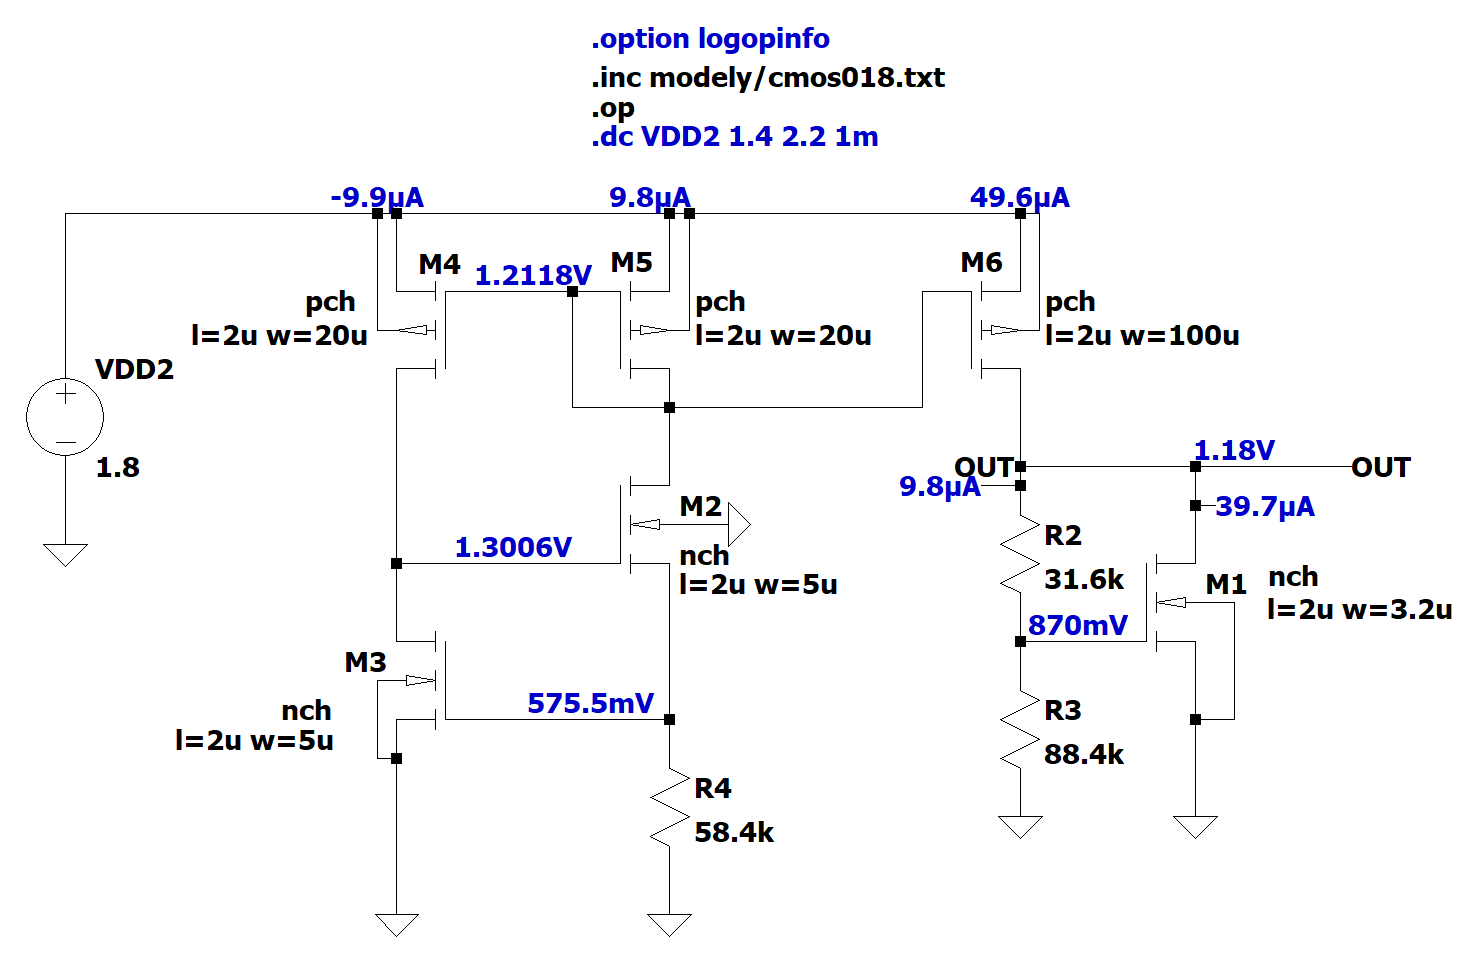
\includegraphics[width=0.9\textwidth]{text/img/LNR-op-sch.png}
    \caption{\label{fig:LNR-op-sch} Zobrazení napětí a proudu ve schématu}
\end{figure}

\vspace{10mm}
\begin{figure}[h!]
    \centering
    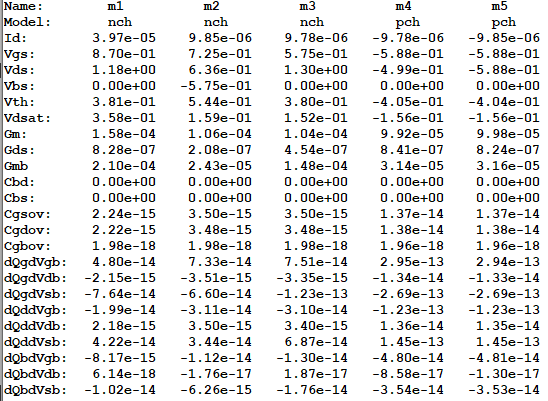
\includegraphics[width=0.9\textwidth]{text/img/LNR-op-ol.png}
    \caption{\label{fig:LNR-op-ol} Pracovní bod tranzistoru}
\end{figure}

\begin{figure}[h!]
    \centering
    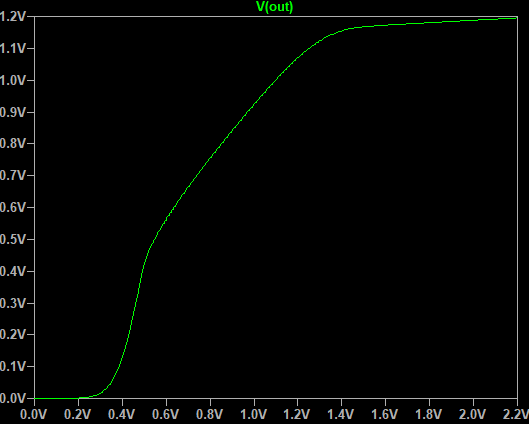
\includegraphics[width=0.9\textwidth]{text/img/LPR_zavislost.png}
    \caption{\label{fig:LNR-zav} Zobrazení napětí a proudu ve schématu}
\end{figure}

\vspace{10mm}
\begin{figure}[h!]
    \centering
    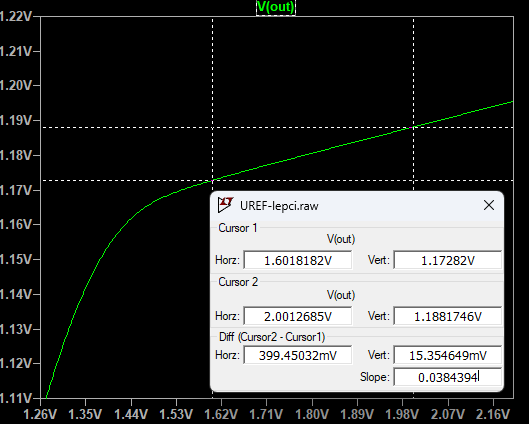
\includegraphics[width=0.9\textwidth]{text/img/LPR-detail_zavislosti.png}
    \caption{\label{fig:LNR-det-zav} Pracovní bod tranzistoru}
\end{figure}

